\subsection{Spectra}\label{sec:spectra}
SunPy aims to provide broad support for solar spectroscopy
instruments.  The variety and complexity of these instruments and
their resultant datasets makes this a challenging goal.  The \texttt{spectra} module implements a
\texttt{Spectrum} class for 1D data (intensity as a function of frequency) and a
\texttt{Spectrogram} class for 2D data (intensity as a function of time and
frequency).  Each of these classes uses a \texttt{numpy.ndarray} object
as its \texttt{data} attribute.  

As with other SunPy data types, the \texttt{Spectrogram} class has been
built so that each instrument initialises using a subclass containing the instrument-specific 
functionalities. The common functionality provided by the base \texttt{Spectrogram} class includes
joining different time ranges and frequencies, performing frequency-dependent background subtraction,
and convenient visualization and sampling of the data.
Currently, the \texttt{Spectrogram} class supports radio spectrograms from the 
\href{http://www.e-callisto.org/}{e-Callisto} \citep{2009EM&P..104..277B}
solar radio spectrometer network and \textit{STEREO}/SWAVES spectrograms \citep{2008SSRv..136..487B}.

Listing \ref{code:spectra} shows how the \texttt{CallistoSpectrogram}
object retrieves spectrogram data in the time range specified taken at
the observatory of interest.  When the data is requested using the
\texttt{from\_range()} function, the object merges all the downloaded
files into a single spectrogram, across time and frequency.
In the example shown, data is provided in two frequency ranges:
20--90\,MHz and 55--355\,MHz.  Since the data are not evenly spaced in
the frequency range, the \texttt{Spectrogram} object linearises the
frequency axis to assist analysis.  The example also demonstrates
the implemented background subtraction method, which calculates
a constant background over time for each frequency channel.
% RJH: Which subtraction method?  If the specifics are irrelevant, cut it.
% RJH: is this better?
%ji to DPS - what is the linearisation that is happening here?
%ji- the linearisation consist in the frequency axis being linear and the 
% data being streched with it.  The frequency normally are not evenly spaced
%ays: I deleted the phrase "based on the values closer to the average" because I don't understand what that means

\begin{listing}[H]
\pythoncode{pycode_spectra.txt}
\begin{center}
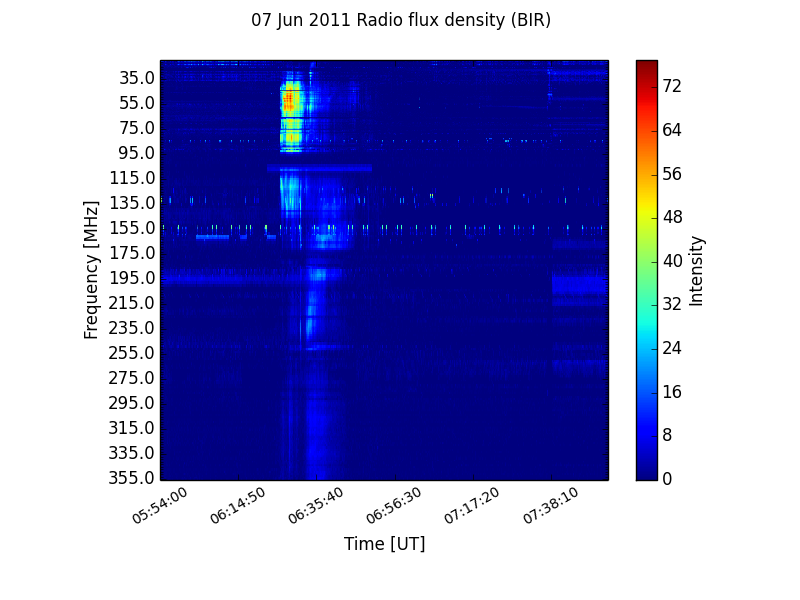
\includegraphics[width=0.8\columnwidth]{callisto_nobg}
\end{center}
\caption{Example of how \texttt{CallistoSpectrogram} retrieves the
  data for the requested time range and observatory, merges it, and
  removes the background signal.  The data requested -- `BIR' -- is
  the code name of the \href{http://www.rosseobservatory.ie}{Rosse Observatory}
  at Birr Castle in Ireland.}
\label{code:spectra}
\end{listing}

